\documentclass[12pt]{article}
\usepackage[utf8]{inputenc}
\usepackage[T1]{fontenc}
\usepackage{lmodern}
\usepackage[margin=1in]{geometry}
\usepackage{setspace}
\usepackage{graphicx}
\usepackage{booktabs}
\usepackage{multirow}
\usepackage{array}
\usepackage{tabularx}
\usepackage{threeparttable}
\usepackage[font=small,labelfont=bf]{caption}
\usepackage{float}
\usepackage{amsmath}
\usepackage[round,authoryear]{natbib}
\usepackage[hidelinks]{hyperref}
\usepackage{pdflscape}

\graphicspath{{figures/}}
% Primitive \input is expandable, so it is safe inside tabular before \bottomrule.
\makeatletter\newcommand{\tabinput}[1]{\@@input #1 }\makeatother
\newcolumntype{L}[1]{>{\raggedright\arraybackslash}p{#1}}
\renewcommand{\arraystretch}{1.15}
\setlength{\tabcolsep}{4pt}

\title{\textbf{The Cabinet and the Countryside:\\ Land, Party, and the State in the Turkish Parliament, 1945--1980}}
\author{[Author names withheld for review]}
\date{}

\begin{document}
\maketitle
\thispagestyle{empty}

\begin{abstract}
\noindent Theories of agrarian politics expect land to divide legislatures: landed elites should defend property, rural deputies should defend the countryside, and land reform should be a contest between classes or regions. Using an original record of every named parliamentary vote on land and agriculture in Turkey from 1945 to 1980 (511 Assembly roll calls and 216,315 deputy votes, linked to biographies of 2,979 deputies and to the speeches of the decisive land debates), we show that this is not how the countryside entered the legislature. Agrarian roll calls were votes of confidence in the cabinet. The same deputies reversed their votes on the same farm agencies when their party entered or left government; exits from the governing party, in 1955 and again in 1970, turned deputies against the cabinet's farm budgets, while exits between opposition parties changed nothing. Farmer and landowner deputies, and deputies from rural provinces, voted like their party colleagues in every era. Landed interests acted through voice and exit instead: they dominated the land debates, stayed away from votes on land distribution while voting openly against land taxes, and left the governing party. Land was redistributed only twice, both times when party competition was absent or suspended. We argue that in strong states agrarian conflict is articulated through the struggle for control of the cabinet rather than through cleavages on the floor, and that this cabinet articulation explains both the weakness of agrarian voting blocs and the authoritarian timing of land reform.

\medskip
\noindent\textbf{Keywords:} political articulation, agrarian politics, land reform, roll calls, state formation, Turkey
\end{abstract}

\newpage
\doublespacing
\setcounter{page}{1}

Few questions have shaped historical sociology as much as the political fate of the countryside. From \citet{moore1966} to \citet{paige1975} and \citet{skocpol1979}, the relation between landlords, peasants, and the state has been treated as a key to the paths that societies take into the modern world, and the question of land---who owns it, who works it, and whether the state will take it from some to give it to others---has been the hinge on which those paths turn. The same question organizes the classic theory of party systems: the cleavage between land and industry is one of the four that \citet{lipset1967} placed at the origin of European parties, and a long line of work since \citet{bates1981} has asked why agrarian majorities so often fail to get what they want from the states they elect.

Underlying these traditions is an assumption about how agrarian conflict enters political institutions. Whether one emphasizes class \citep{moore1966}, sector \citep{bates1981}, or the center and periphery of a state \citep{mardin1973}, landed interests are expected to appear in the legislature as a recognizable bloc: deputies who own land or represent rural constituencies should vote against redistribution, defect from their parties when land is at stake, and line up along a dimension of conflict that can be read off their votes. Recent sociological work on political articulation has loosened the first part of this assumption, showing that parties do not simply translate social divisions but actively make, suppress, and reshape them \citep{desai2002,deleon2009,deleon2015,mudge2014,eidlin2016}. But articulation theory, too, has mostly asked which social cleavages parties choose to politicize, not whether the conflict over land is fought on the floor at all.

In this article we examine that assumption with an unusually complete record. We assembled every named vote on land and agriculture in the Turkish Grand National Assembly from the passage of the 1945 land distribution law to the military coup of 1980---a period that covers a single-party regime, a two-party decade, a fragmented multiparty system, and a period of military tutelage---and linked each vote to the biographies of the deputies who cast it and, for the decisive land laws, to the speeches they gave. Turkey is a strategic case. Its party system was born in a dispute over land: the four deputies who founded the Democrat Party, the party that would end single-party rule in 1950, were among the most prominent critics of the 1945 law, and the received account treats the law as the moment when landed interests broke with the Republican People's Party \citep{karpat1959,keyderpamuk1984}. Land reform returned to the agenda in every decade that followed, and it passed again only once, in 1973, under military supervision. If landed interests shaped legislative conflict anywhere, they should have done so here.

They did not, at least not in the way theories of agrarian politics expect. Across thirty-five years, agrarian roll calls behaved as votes of confidence in the cabinet. The same deputies voted for and against the same farm agencies as their parties entered and left government. Deputies who left the governing party turned against its farm budgets; deputies who moved between opposition parties did not change their votes. Farmers, landowners, and deputies from rural provinces voted exactly like their party colleagues. Landed deputies were not silent---they dominated the debates on land---but their opposition took the form of voice in debate, absence from the vote, and exit from the party, never a recorded vote against their own side. And land was redistributed only when there was no competing party to vote against it.

We argue that these regularities reflect what we call \emph{cabinet articulation}: in states where the executive controls the agenda and the resources that agrarian policy distributes, agrarian conflict is articulated as a struggle over control of the cabinet rather than as a cleavage among deputies. This argument extends the recent state-centered account of party formation by \citet{rohr2025} \citep[see also][]{slez2007,shefter1994}, who show that the first American parties coalesced around the organizational affordances of the state rather than around social cleavages, to the most classic of substantive cleavages. It also helps resolve a puzzle in the literature on land reform: why redistribution so often comes from authoritarian or tutelary regimes \citep{huntington1968,albertus2015}. If landed interests in competitive legislatures act through voice, absence, and exit rather than through votes, land reform requires not a defeat of landed deputies on the floor but the suspension of the party competition that gives exit its force.

\section*{Theories of Agrarian Conflict in Legislatures}

\subsection*{Sociology: Land as a Cleavage}

Sociological accounts of agrarian politics begin from the structure of rural society. In the comparative-historical tradition, the political orientation of landed classes---their dependence on labor-repressive agriculture, their alliances with the bourgeoisie or the crown---determines whether democracy survives and whether land is redistributed \citep{moore1966,paige1975}. In the party-systems tradition, the conflict between land and industry is one of the critical cleavages that national revolutions bequeathed to modern party systems, and the degree to which agrarian parties formed depended on how this cleavage intersected with others \citep{lipset1967}. Both traditions imply that agrarian conflict should be visible in parliament as a division among deputies along social lines. We call this the \emph{landed cleavage} hypothesis: deputies who own or work land should vote differently on land than others, and especially against redistribution and land taxation, regardless of party.

A second, spatial version of the cleavage argument locates the division not in deputies' own class positions but in their constituencies. Theories of urban bias and of the collective action of farmers \citep{olson1965,bates1981} imply that deputies representing rural constituencies should defend agricultural prices, credit, and land against urban majorities. In Turkey, the most influential version of this argument is \citeauthor{mardin1973}'s (\citeyear{mardin1973}) account of a confrontation between a bureaucratic center and a rural periphery, in which the Democrat Party and its successors gave voice to provincial notables and peasants against the Kemalist state. We call this the \emph{rural constituency} hypothesis: deputies from rural provinces, or from provinces hit by agrarian distress, should form a bloc on agrarian votes.

A third account comes from the literature on land reform. Here the question is not whether landed interests are represented but whether they can block redistribution. \citet{albertus2015} shows that land reform is far more common under autocracy than democracy, because democratic institutions give landed elites the veto points they need, unless the ruling coalition splits from them. We call this the \emph{landed veto} hypothesis: in competitive legislatures, landed deputies should vote down redistribution, and reform should pass only when they are outvoted or excluded.

\subsection*{Articulation: Parties Make Cleavages}

The articulation approach rejects the idea that parties simply express pre-existing social divisions. Parties ``naturalize'' some divisions and suppress others, building blocs out of heterogeneous materials \citep{deleon2009,deleon2015}. The approach was developed partly on the Turkish case, where \citet{deleon2009} and \citet{tugal2009} show how parties articulated a religious-secular divide that was not given by social structure. For agrarian politics, articulation theory implies that land becomes a partisan issue to the extent that parties make it one, and that parties may also work to keep land off the agenda. We call this the \emph{articulated cleavage} hypothesis: land votes should divide parties when, and only when, party leaders politicize land, and deputies should follow their parties' articulation rather than their own positions. Articulation theory also leaves room for a radical flank: a party that politicizes land more radically than others may pull the center left or force concessions \citep{haines1984}.

\subsection*{Political Science: The Cabinet and the Agenda}

Political scientists have tended to see parliamentary parties as endogenous organizations that solve the problems of office holders. In parliamentary systems, the defining problem is the survival of the cabinet. \citet{cox1987} shows that cohesive voting in the British House of Commons emerged as the cabinet came to control the legislative agenda and as votes on government measures became votes on the government itself; \citet{huber1996} shows how executives use procedural instruments to turn policy votes into confidence votes; and \citet{cox2005} treat majority parties as cartels that control what reaches the floor. In this view, what deputies vote on matters less than who controls the government that proposed it. We call this the \emph{cabinet} hypothesis: on agrarian as on other votes, deputies should vote with or against the government according to whether their party holds cabinet office, and should change their votes when that status changes.

\subsection*{A State-Centered Synthesis: Cabinet Articulation}

These traditions are usually treated as rivals. We propose instead that they describe different moments in a single process, and that what connects them is the state. \citet{rohr2025} argue that the first American party system formed not around cleavages but around the organizational affordances of the modern state---the offices and procedures that determined who would control positions in an expanding administration. Their argument concerns formal, structural issues. Ours concerns substantive ones. In states that distribute agrarian resources through executive agencies---grain boards, state farms, irrigation authorities, land-reform administrations---every vote on agriculture is also a vote on the cabinet that runs those agencies. Under these conditions, parties have strong incentives to articulate agrarian conflict as a question of cabinet control, and deputies have strong incentives to follow. Landed interests do not disappear; they move to the places where voting on the cabinet does not constrain them: debate, absence, and party exit \citep{hirschman1970}.

This argument yields several implications that distinguish it from the alternatives. First, agrarian votes should follow cabinet status within deputies, across regimes and governing parties. Second, party exits should change votes only when they move deputies across the line between government and opposition; an exit that leaves deputies in opposition should not. Third, deputies' land, occupation, and constituency should not predict their votes within party, though landed deputies may speak more. Fourth, opponents of land distribution should prefer absence to a recorded no, because a vote against giving land to peasants is costly with rural electorates, while opposition to land taxes can be recorded openly. Fifth, redistribution should pass when party competition is absent or suspended, because only then does the exit option lose its force. Table~\ref{tab:hyp} summarizes the hypotheses and the indicators by which we evaluate them.

\begin{table}[p]
\centering
\caption{Hypotheses and Empirical Indicators}
\label{tab:hyp}
\small
\begin{tabular}{L{2.6cm}L{4.6cm}L{8.2cm}}
\toprule
Hypothesis & Theory & Empirical indicators \\
\midrule
Landed cleavage & Deputies' own class position on land shapes their votes (Moore; Lipset and Rokkan) & Farmer and landowner deputies vote differently from party colleagues on land, land taxes, and farm benefits; defection concentrated on redistribution \\
Rural constituency & Deputies defend rural constituencies against urban majorities (Bates; Mardin) & Rural-province deputies and deputies from provinces hit by harvest failure vote as a bloc; a regional or rural dimension appears in the vote space \\
Landed veto & Landed elites block redistribution in democracies (Albertus) & Land reform defeated by recorded votes of landed deputies; passage when they are outvoted \\
Articulated cleavage & Parties politicize or suppress land (De Leon, Desai, and Tu\u{g}al) & Land votes divide parties when leaders politicize land; a radical party shifts outcomes or the center \\
Cabinet & Votes are votes on the government (Cox; Huber) & Votes follow cabinet status within deputies; exits change votes only when they cross the government--opposition line \\
Cabinet articulation & Agrarian conflict is articulated as cabinet control; landed interests act through voice and exit (this article) & All cabinet indicators; no landed or rural vote within party; landed voice in debate; absence on distribution but open no on taxes; redistribution only without competition \\
\bottomrule
\end{tabular}
\end{table}

\section*{The Case: Land and Party in Turkey, 1945--1980}

Turkey entered the postwar period as a single-party republic in which the Republican People's Party (CHP) governed a largely agrarian society through a strong bureaucratic state \citep{heper1985,keyder1987}. In 1945, as the regime prepared a controlled opening to multiparty politics, the government introduced the Law on Providing Land to Farmers (\textit{Çiftçiyi Topraklandırma Kanunu}). Its seventeenth article allowed the expropriation of land worked by sharecroppers and tenants down to small holdings. The bill was fiercely debated; during the debate four CHP deputies---Celâl Bayar, Adnan Menderes, Fuat Köprülü, and Refik Koraltan---submitted their memorandum calling for political liberalization, and in January 1946 they founded the Democrat Party (DP). The standard account treats the land law as the issue on which landed notables, Menderes among them, broke with the single party \citep{karpat1959,keyderpamuk1984,zurcher2004}.

The DP won the 1950 elections and governed for a decade, overseeing agricultural mechanization, rising crop prices, and an expansion of state credit and agencies in the countryside \citep{keyder1987,ahmad1977}. It split twice: in 1948, while still in opposition, when dissidents founded the Millet Partisi (MP), and in 1955, in government, when dissidents founded the Hürriyet Partisi (HP). The military coup of 1960 ended DP rule and introduced a bicameral parliament with proportional representation. In the 1960s and 1970s, the Justice Party (AP), heir to the DP, alternated in power with the CHP, coalitions with smaller parties, and in 1971--73 cabinets formed under the supervision of the military after the memorandum of March 12, 1971. Land reform returned repeatedly: the CHP-led coalition of İsmet İnönü introduced a land reform bill in 1965; the Workers' Party of Turkey (TİP), which entered parliament the same year, demanded ceilings on landholding; and in 1973, after TİP had been closed by the courts, the military-supervised cabinets passed the Land and Agrarian Reform Law with the votes of the AP.

Three features make this case useful for adjudicating theories of agrarian politics. First, land was a salient and recurrent issue, so a landed cleavage had repeated opportunities to appear. Second, the period offers within-case variation in the factors theories emphasize: the regime (single party, competitive, tutelary), the governing party (CHP, DP, AP, coalitions), and the presence of a radical flank. Third, the Turkish parliament recorded named votes on the final passage of laws and on budgets throughout the period, and in the 1960s and 1970s also on articles and motions, so that the same kind of record exists under very different political conditions.

\section*{Data and Methods}

\subsection*{The Record}

Our data come from the official minutes of the Turkish Grand National Assembly (\textit{Tutanak Dergisi}), which print the full list of deputies voting yes, no, and abstaining and of those not taking part in each named vote. We identified named votes on land and agriculture in three steps. For 1961--80 we searched the minutes of the National Assembly (\textit{Millet Meclisi}) and the Senate for all named votes on land, agricultural credit and prices, commodity boards, forests, irrigation, state farms, and the budgets and accounts of the agencies responsible for them. For 1943--60 we located every printed vote result in a page-level text corpus of the minutes (the GNACT corpus; supplement Part A), identifying 1,872 named votes, of which 143 concern agriculture (1946--60) and 57 fall in the period around the 1945 land law. We then retrieved the original page images and parsed the name lists with a layout parser that reconstructs columns, province headings, and section headings. The minutes' vocabulary changed over time (\textit{Kabul etmiyenler} and \textit{Oya katılmıyanlar} in 1945, \textit{Reddedenler} and \textit{Reye iştirak etmiyenler} in the 1950s), and the 1945 lists print initials rather than full names, so the parser was adapted for each era and every list was checked against the printed tallies.

The resulting record contains 511 Assembly roll calls and 216,315 deputy votes: 54 votes from 1945, 135 agrarian votes from 1946--60, and 322 from the National Assembly in 1961--80 (the Senate's 245 votes are analyzed in the supplement but excluded here because senators' parties are not observed). Table~\ref{tab:eras} describes the record by era. Deputies were linked to the Turkish Political Elites Dataset by legislative term, province, and name; 85 percent of names were matched in 1945 and 89.5 percent in 1946--60, and the 73 land votes of 1961--80 were verified by hand against the original pages. Unmatched names leave a deputy's cell empty rather than miscoded; the online supplement (Part A, Table A2) reports accuracy in detail.

\begin{landscape}
\begin{table}[p]
\centering
\begin{threeparttable}
\caption{The Record of Agrarian Roll Calls by Era, 1945--1980}
\label{tab:eras}
\small
\begin{tabular}{llrrrrrrrrr}
\toprule
 & & \multicolumn{3}{c}{Record} & \multicolumn{3}{c}{All roll calls (\%)} & \multicolumn{3}{c}{Contested roll calls} \\
\cmidrule(lr){3-5}\cmidrule(lr){6-8}\cmidrule(lr){9-11}
Era & Regime & Roll calls & Deputy votes & Deputies & Contested & Not yes & Took part & Gov.\ yes (\%) & Opp.\ yes (\%) & Premium \\
\midrule
\tabinput{tables/t2_eras.tex}
\bottomrule
\end{tabular}
\begin{tablenotes}\footnotesize
\item \textit{Note:} Turkish Grand National Assembly (1945--60) and National Assembly (1961--80). \textit{Contested}: the losing side holds at least 5 percent of votes cast. \textit{Not yes}: no and abstain as a share of votes cast. \textit{Took part}: share of listed deputies casting a vote. \textit{Gov.\ yes} and \textit{Opp.\ yes}: yes among votes cast on contested roll calls by deputies whose party did and did not hold cabinet posts. \textit{Premium}: mean over contested roll calls of the difference between government and opposition yes shares. Ministers, presiding officers, and deputies on leave are excluded. The 1946--50 premium rests on four contested roll calls.
\end{tablenotes}
\end{threeparttable}
\end{table}
\end{landscape}

\subsection*{Measures}

Our outcome is a deputy's choice on a roll call, coded as yes among votes cast (yes, no, or abstain) and as taking part (casting any vote). A deputy is in government when his or her party holds cabinet posts on the date of the vote; party at the vote follows each deputy's party switches by date. For deputies' land and occupation we coded the biographies printed in the parliament's official album (\textit{TBMM Albümü 1920--2010}; supplement Part A), which record each deputy's education, occupation, and career; 7,355 biographies covering 1920--80 were matched to the elites dataset at rates of 97 to 100 percent in every term. A deputy is coded as a farmer or landowner when the biography lists farming, a farm, land, or livestock as an occupation (\textit{çiftçi}, \textit{çiftlik sahibi}, \textit{ziraatçı}, \textit{arazi sahibi}, \textit{hayvancılık}); the share ranges from 9 percent of deputies before 1946 to 18 percent in the 1950s. Menderes, for instance, is listed as \textit{çiftçilik} and Emin Sazak as \textit{ziraatçı}. Province characteristics come from the elites dataset, and provincial harvest shocks from yields relative to each province's trend. For the land debates of 1945 and 1950 we split the minutes into speaker turns and matched speakers to the roster; all quotations were checked against the original page images.

\subsection*{Designs and Estimands}

We use four designs, each with an explicit estimand. First, we describe the vote space of each term with a two-dimensional item-response model \citep{poole1997,clinton2004}, fitted to roll calls whose lists match their tallies, and we summarize partisanship in each era by the \emph{government premium}: the mean, over contested roll calls, of the difference between the yes shares of government and opposition deputies. Second, to identify the effect of cabinet status on votes, we exploit changes in status within deputies. For the 1950 turnover, we compare deputies elected in both 1946 and 1950 who remained in the DP (which moved from opposition to government) with those who remained in the CHP (which moved the other way), on the same roll calls; for 1961--80, we use the DID$_M$ estimator of \citet{dechaisemartin2020}, which compares deputies whose status switches between consecutive periods with those whose status does not, and report a placebo for periods without switches. Third, we treat the four parliamentary splits of the period as a two-by-two comparison: two exits from the governing party (1955, 1970) and two exits between opposition parties (1948, 1967). For each, the estimand is the difference-in-differences in yes between leavers and stayers before and after the split, with inference by Fisher randomization over which deputies are labelled as leavers \citep{imbens2015}. Fourth, we estimate the effect of deputies' occupation and constituency within party and roll call, with party-by-roll-call fixed effects and standard errors clustered by deputy, so that a farmer is compared with party colleagues voting on the same question. We complement these designs with process tracing of the land laws \citep{collier2011} and a controlled comparison of the periods in which land reform reached a vote \citep{slater2013}.

\section*{Analyses}

\subsection*{One Dimension, Many Splits}

We begin with the shape of the vote space. If land formed a cleavage of its own, agrarian votes should require a second dimension, and that dimension should be associated with deputies' social positions. Figure~\ref{fig:maps} shows the estimated positions of deputies in the two National Assemblies in which the most important splits occurred. In both, the first dimension separates the governing party from the opposition, and the model classifies 97 to 98 percent of individual votes correctly. The second dimension does not separate rural from urban deputies or the east from the west of the country: its within-party correlations with the rural share of the province and with an eastern province are at most 0.10 in absolute value in every term. The two panels also preview the comparison of party exits below. In 1965--69, the CHP deputies who left in 1967 to found the Güven Partisi---a split from one opposition party to another---are indistinguishable from the rest of the CHP on the first dimension (mean $-0.69$ against $-0.64$). In 1969--73, the AP deputies who left the governing party to found the Demokratik Parti sit far from the governing party's tight cluster and close to the opposition (mean $-0.38$ against $+0.37$). Because positions are estimated over the whole term, this distance reflects the votes they cast after leaving; Table~\ref{tab:designs} identifies that change directly.

\begin{figure}[t]
\centering
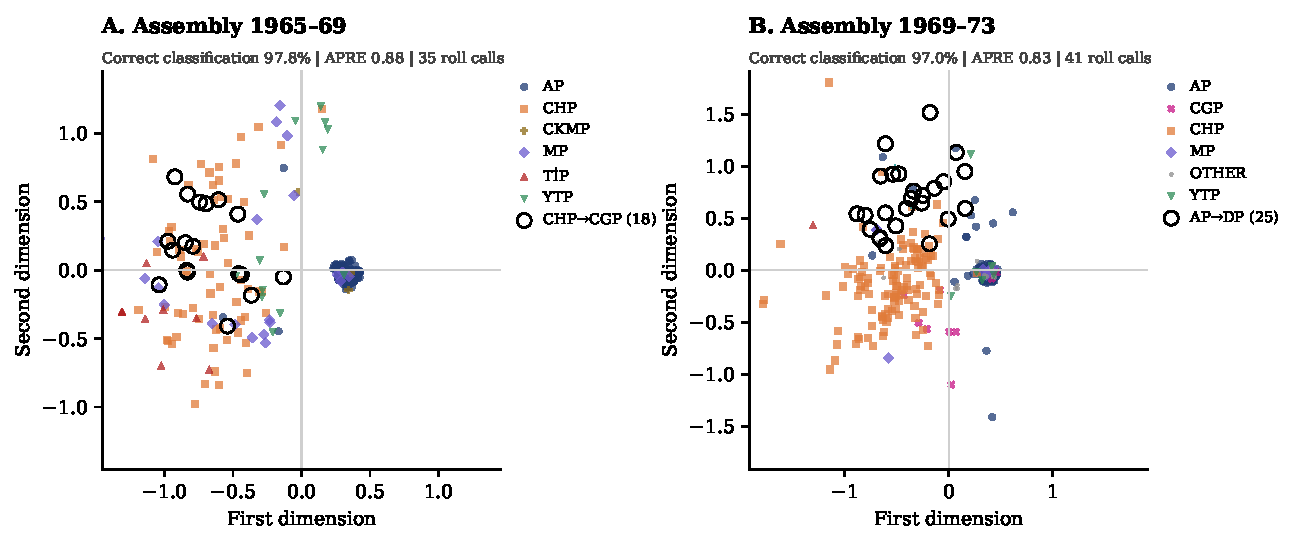
\includegraphics[width=\textwidth]{fig1_split_maps.pdf}
\caption{Estimated Positions of Deputies, National Assembly 1965--69 and 1969--73}
\label{fig:maps}
\begin{minipage}{\textwidth}\footnotesize\singlespacing
\textit{Note:} Two-dimensional item-response estimates fitted to agrarian roll calls whose name lists match their tallies. Each point is a deputy, by party at the start of the term. Circled: deputies who later left their party (Panel A: CHP to Güven Partisi, 1967; Panel B: AP to Demokratik Parti, 1970). Fit statistics are reported above each panel. Other terms appear in supplement Figure A4.
\end{minipage}
\end{figure}

The dominance of a single government--opposition dimension holds across all seven eras (Table~\ref{tab:eras} and Figure~\ref{fig:eras}). Where there was competition, government deputies voted yes on contested agrarian roll calls 92 to 100 percent of the time and opposition deputies 16 to 49 percent of the time, for a premium between 0.42 and 0.84. The premium was smallest, 0.31, under the military-supervised cabinets of 1971--73, to which we return below. The intensity of conflict, by contrast, grew with competition: no agrarian roll call was contested in 1945, 11 percent were under the CHP government of 1946--50, 24 percent under the DP, and 58 percent under the AP majority of 1965--71, before falling to 30 percent under tutelage and rising again to 47 percent after 1973.

\begin{figure}[t]
\centering
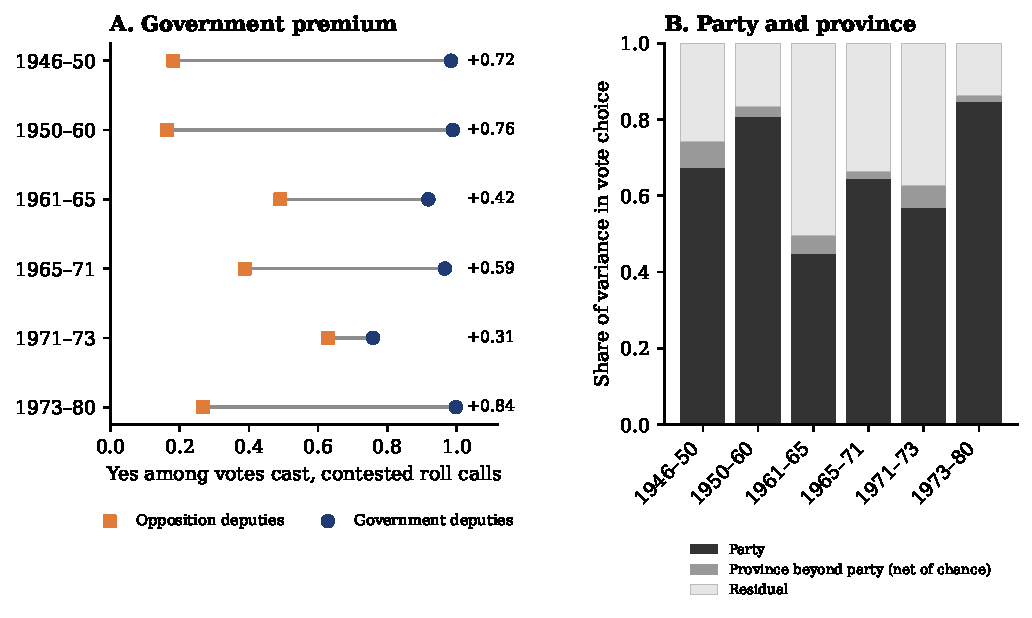
\includegraphics[width=\textwidth]{fig2_eras.pdf}
\caption{Government Premium and Partisan Conflict on Agrarian Roll Calls by Era}
\label{fig:eras}
\begin{minipage}{\textwidth}\footnotesize\singlespacing
\textit{Note:} Panel A: yes among votes cast on contested roll calls by government and opposition deputies; the number is the government premium (Table~\ref{tab:eras}). Panel B: share of roll calls that were contested and share of all votes cast that were not yes. 1945 had no contested roll call and no opposition party.
\end{minipage}
\end{figure}

\subsection*{The Cabinet, Not the Countryside}

Descriptive premiums cannot distinguish the cabinet hypothesis from the possibility that parties with different agrarian programs simply take turns in government. The within-deputy designs in Table~\ref{tab:designs} address this. The 1950 turnover provides the sharpest test: the same 68 deputies, who kept their party, voted on the same kinds of agrarian roll calls before and after their party's status changed. DP deputies who had voted yes on 5 percent of contested agrarian roll calls in opposition voted yes on 100 percent in government; CHP deputies fell from 99 to 40 percent. The difference in differences, which adds the two reversals together, is 1.54, and no random reassignment of party labels among these deputies produces a value as large ($p<.001$). In 1961--80, where coalitions and technocratic cabinets blur status, the DID$_M$ estimate of entering government is 0.41 (95 percent CI 0.11 to 0.50), with a placebo of 0.002 in periods without switches; entering government also raised participation by 0.22.

\begin{table}[t]
\centering
\begin{threeparttable}
\caption{Within-Deputy Designs: Cabinet Status and Party Exit}
\label{tab:designs}
\footnotesize
\begin{tabular}{lL{4.9cm}crrrL{2.9cm}}
\toprule
Design & Group & Deputies & Before (\%) & After (\%) & Estimate & Inference \\
\midrule
\tabinput{tables/t3_designs.tex}
\bottomrule
\end{tabular}
\begin{tablenotes}\footnotesize
\item \textit{Note:} Outcome: yes among votes cast. Panel A, 1950: deputies elected in both 1946 and 1950 who kept their party; contested agrarian roll calls; the estimate adds the two groups' changes. 1961--80: DID$_M$ estimator \citep{dechaisemartin2020}; 95 percent bootstrap interval clustered by deputy; placebo for periods without a switch. Panel B: difference in differences between leavers and stayers, before and after the split. Outcomes: contested agrarian roll calls (1948), agency budgets (1955, 1970), contested agency budgets (1967). ``Deputies'' gives leavers / stayers. RI: Fisher randomization over deputies, 5,000 draws.
\end{tablenotes}
\end{threeparttable}
\end{table}

The party exits offer a second, independent test (Table~\ref{tab:designs}, Panel B, and Figure~\ref{fig:exits}). All four splits were driven by disputes that had nothing to do with agrarian budgets, but only two of them moved deputies across the line between government and opposition. In both, the effect was large and immediate. The DP deputies who left to found the Hürriyet Partisi in 1955 had voted for every agency budget before the split; afterward they voted for 48 percent, while the stayers remained at 100 percent ($-0.52$, $p<.001$). Fifteen years later, under a different constitution and with a different party, the AP deputies who left to found the Demokratik Parti fell from 100 percent to 14 percent ($-0.83$, $p<.001$). The two exits between opposition parties produce nothing: the DP deputies who left for the Millet Partisi in 1948 changed their votes by $+0.10$ ($p=.23$), and the CHP deputies who founded the Güven Partisi in 1967 by $-0.04$ ($p=.46$). Leaving a party does not change how deputies vote on agriculture; leaving the government does.

\begin{figure}[t]
\centering
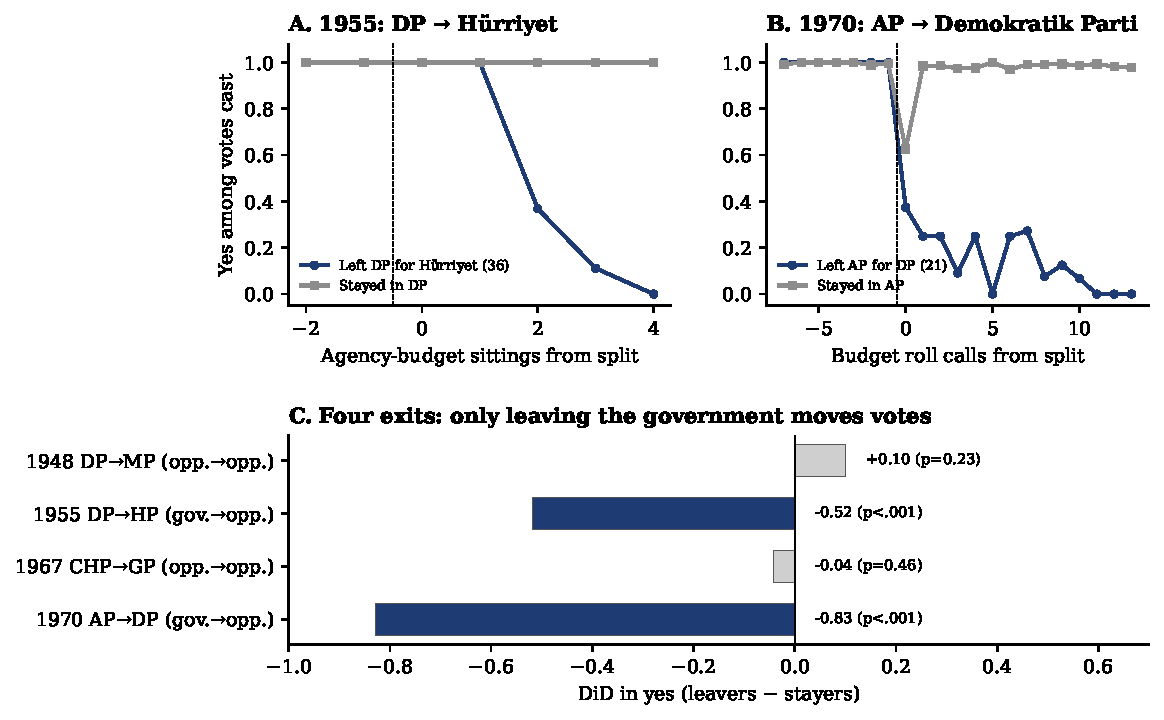
\includegraphics[width=\textwidth]{fig3_exits.pdf}
\caption{Party Exits and Votes on Agrarian Agency Budgets}
\label{fig:exits}
\begin{minipage}{\textwidth}\footnotesize\singlespacing
\textit{Note:} Panels A and B: yes among votes cast on agency budgets by leavers and stayers, by roll call relative to the split (dashed line). Panel C: difference-in-differences estimates for all four exits, with Fisher randomization $p$-values; dark bars are exits from the governing party.
\end{minipage}
\end{figure}

One exit preceded its own cause in a revealing way. Six months before the AP split, the future founders of the Demokratik Parti had already broken with their party on a single issue: the 1970 property tax, which extended taxation to land. A third of them voted against it while only 1 percent of the stayers did (Fisher's exact $p=5\times10^{-9}$). This is the one place in our record where a substantive agrarian position anticipates partisan behavior, and the issue is not the distribution of land but its taxation. We return to this asymmetry below.

\subsection*{Land, Constituency, and the Vote}

If agrarian votes are votes on the cabinet, deputies' own relation to land should not predict their votes once party and roll call are held constant. Table~\ref{tab:social} reports these within-party comparisons. Farmer and landowner deputies voted on contested agrarian roll calls exactly as their party colleagues did: the difference is $-0.002$ (SE 0.007) in 1946--60 and $+0.002$ (SE 0.009) on land and land-tax votes in 1961--80, and the estimate is within two standard errors of zero in each of the six competitive eras (supplement Table A4, Panel C). The same holds for constituencies: a one standard deviation increase in the rural share of a deputy's province changes the probability of a yes vote by less than half a percentage point in either period, and deputies from provinces hit by a harvest shock were no more likely to turn out for farm benefits. These are precise nulls, estimated on hundreds of farmer deputies and tens of thousands of votes. The only behavioral difference is that farmer deputies took part slightly less often in land votes ($-0.030$, SE 0.015).

\begin{table}[t]
\centering
\begin{threeparttable}
\caption{Land, Constituency, and Votes within Party}
\label{tab:social}
\footnotesize
\begin{tabular}{L{4.1cm}L{4.8cm}lrr}
\toprule
Deputy characteristic & Outcome & Period & Estimate (SE) & Deputies \\
\midrule
\tabinput{tables/t4_social.tex}
\bottomrule
\end{tabular}
\begin{tablenotes}\footnotesize
\item \textit{Note:} Panel A: differences between deputies with and without the characteristic, within party and roll call (party $\times$ roll-call fixed effects), standard errors clustered by deputy; ``Deputies'' counts deputies with the characteristic. Farmer or landowner: occupation in the \textit{TBMM Albümü} lists farming, a farm, land, or livestock. Harvest shock: provincial yield relative to trend, 1968--80. Panel B: 1945 land law. Excess absence compares each deputy's absence on the land law with his own absence on the other 53 votes of 1945, relative to other deputies; $p$ from randomization over votes. Shares of speech: speaker turns in the debates of May 14--21 and June 4--11, 1945.
\end{tablenotes}
\end{threeparttable}
\end{table}

Landed deputies were not passive, however. They spoke. In the 1945 land debate, the 41 farmer and landowner deputies made up 9 percent of the house but accounted for 16 percent of speakers and 23 percent of the words spoken; the 14 deputies who would later sit for the DP, 3 percent of the house, accounted for 16 percent. What they said was unambiguous. Menderes called the bill's plan for family farms a copy of the National Socialist hereditary farm law; Cavit Oral, a Seyhan (Adana) landowner who headed the province's farmers' union, protested that Article 17 ``recognizes no limit in land''; and Emin Sazak told the assembly that ``if I denied that my tie to land affects my speech, I would be lying'' (supplement Table A3). Yet the law passed by 345 votes to none. Not a single deputy recorded a vote against it.

\subsection*{Voice, Absence, and Exit}

How, then, did the opponents of the 1945 law act? The received account holds that the future DP founders boycotted the land law. Our record shows something different (supplement Figure A1). On May 29, 1945, Bayar, Menderes, Koraltan, Köprülü, and Sazak cast the only five votes against the government's budget, which the prime minister had made a question of confidence. From that day they stopped voting almost entirely: they were absent from 91 percent of the votes that followed, including the land law two weeks later. Measured against their own absence on the other votes of those months, the land law is not distinctive ($p=.18$ over 39 votes). The founders did not single out the land law. They withdrew from the single party's votes in general, and broke cover only to vote against budgets.

This pattern---voice in debate, absence from the vote, and recorded opposition only on the cabinet's budget---recurs throughout the period. Figure~\ref{fig:land} shows, for each of the key land votes of 1950--73, how the party that opposed the bill behaved, measured as its attendance relative to its own attendance on other agrarian votes in the same era. On every law that distributed or registered land, the opposing side stayed away: the DP attended the CHP's 1950 dilution of the land law and its titling law at 0.69 and 0.38 of its usual rate; the CHP attended the DP's 1955 amendment at 0.28, the AP's 1966 titling amendment at 0.13, and the 1973 land reform law at 0.04, when 2 of its 101 listed deputies took part. On every vote that taxed land, by contrast, the opposing side attended at or above its usual rate and voted no: 83 percent of present AP deputies on the 1964 land tax, 96 percent of CHP deputies on the 1970 property tax, and all DP deputies on the 1972 amendment. The single exception confirms the logic. In February 1965 the AP could defeat the motion that would have sent İnönü's land reform bill to a joint committee; it turned out at 1.65 times its usual rate, voted no almost unanimously, and won by 167 to 157.

\begin{figure}[t]
\centering
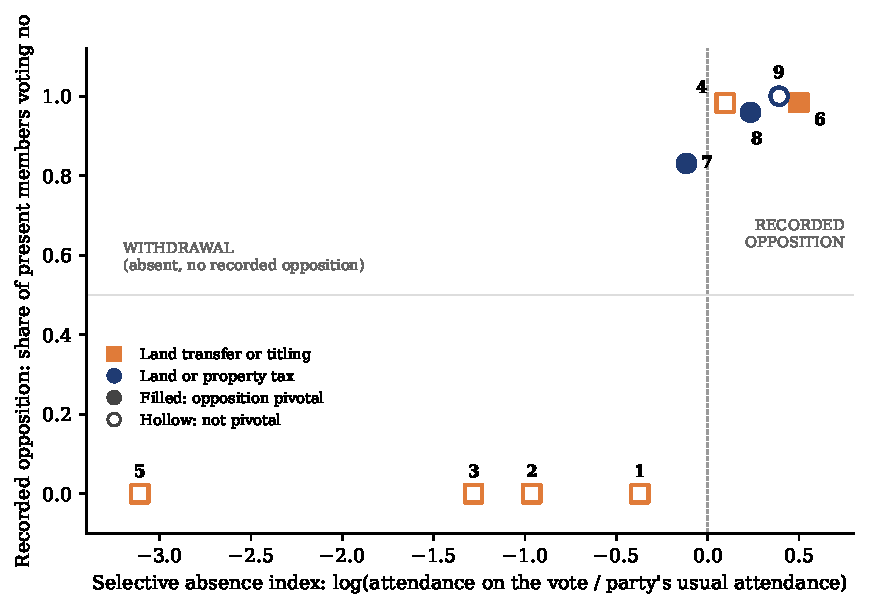
\includegraphics[width=.9\textwidth]{fig4_land_attendance.pdf}
\caption{How Opponents Acted on Key Land Votes, 1950--1973}
\label{fig:land}
\begin{minipage}{\textwidth}\footnotesize\singlespacing
\textit{Note:} For each vote, the attendance of the party that opposed the bill (in parentheses), divided by that party's attendance on the other agrarian roll calls of the same era (1 = usual attendance; log scale). Labels give the share of present members voting no. Distribution: laws that transfer or register land. Taxation: laws that tax land or property. The 1965 motion, which killed the government's land reform bill, was the only distribution vote the opposition could win.
\end{minipage}
\end{figure}

The asymmetry between distribution and taxation is what a theory of cabinet articulation would expect. A recorded vote against giving land to peasants is costly with rural electorates; a recorded vote against taxing land is not. Opponents of redistribution therefore record their opposition only when they can win, and distributive measures that no one opposes on the record pass with the near-unanimity that theories of legislative universalism predict \citep{weingast1979}. Otherwise they leave the floor to the government and fight elsewhere---in debate, in the committee rooms where bills are drafted, and, when the stakes are high enough, by leaving the party.

The 1950 amendment shows where that elsewhere was. Two months before the elections that would end its rule, the CHP itself diluted the 1945 law. The minister who presented the amendment was Cavit Oral, the most persistent critic of Article 17 in 1945. A CHP deputy told the assembly that the delegates at the party's own congress had ``all at once attacked articles 15, 16, 17.'' The fifteen deputies who voted against the dilution all sat on the CHP benches or with it, among them Şevket Raşit Hatipoğlu, the agriculture minister who had carried the 1945 law and who now called it ``the only legacy of honor I can leave my children.'' The landed critics of 1945 had not been defeated by a vote. They had rewritten the law from inside the governing party, with one of them in the cabinet.

\subsection*{When Land Was Redistributed}

Land reform reached a recorded vote in five moments, and passed in two: June 1945 (345 to 0) and June 1973 (238 to 5). Table~A4 (Panel A) in the supplement sets out the comparison. What the two passages share is not a weakened landed class, a radical flank, or a reformist party, but the absence of a competing party that could vote against the cabinet. In 1945 the regime was a single party, and its dissidents had withdrawn. In 1973 the cabinets were formed under military supervision after the memorandum of 1971, and partisan conflict on the floor had collapsed: the distance between the AP and CHP yes shares on agrarian roll calls fell by 0.38 after the memorandum, a drop larger than at 97 percent of placebo break dates (supplement Figure A2). The AP, whose deputies had voted 2 to 127 against İnönü's land reform motion in 1965, voted 198 to 1 for the 1973 law.

Under open competition, by contrast, every governing party used land policy for its own coalition: the CHP diluted its law before an election, the DP and the AP passed titling laws that confirmed possessors' claims, and İnönü's bill was killed by a mobilized opposition. Nor did the radical flank change this. The Workers' Party, which proposed ceilings of 100 dönüm of dry and 20 of irrigated land, was pivotal on none of the 78 roll calls of the 1965--69 Assembly; its ceiling amendments were rejected by a show of hands that left no record; and the CHP deputies who left the party in 1967, in reaction to its turn toward the left, did not change their votes (supplement Table A4, Panel B). Reform came only after the radical party had been closed and competition suspended. The pattern is consistent with the finding that land reform is more common under autocracy \citep{albertus2015}, but the mechanism our record reveals is different from a landed veto: what the suspension of competition removed was not landed votes against reform, which were never cast, but the exit option that made the cabinet's agrarian policy hostage to the next election.

\section*{Discussion}

We began with an assumption shared by many theories of agrarian politics: that the conflict over land enters the legislature as a cleavage among deputies. Across thirty-five years and very different regimes, we find little evidence for it in Turkey's parliament. The deputies' own land, their constituencies, and the fortunes of their provinces' harvests do not predict their votes once party and roll call are held constant. Agrarian roll calls instead behaved as votes on the cabinet, and landed interests appeared in other forms: in debate, in absence, and in party exit. We draw three broader implications.

\subsection*{Cabinet Articulation}

First, our findings extend the state-centered account of party formation. \citet{rohr2025} show that the first American parties coalesced around the organizational affordances of the state, and that partisanship was strongest on structural questions about the rules of the game. In Turkey, the most classic of substantive cleavages was absorbed into the same logic. The state did not merely provide offices for parties to compete over; it ran the grain board, the state farms, the irrigation authority, and the land-reform administration whose budgets made up most of our record. Every vote on these agencies was a vote on the government that controlled them, and parties articulated agrarian conflict accordingly. This is articulation in the sense of \citet{deleon2009}---parties actively shaped which divisions were expressed on the floor---but the division they articulated was not between social groups. It was between those inside and outside the cabinet. We call this cabinet articulation and suggest that it should be strongest where three conditions hold: a parliamentary executive that controls the agenda \citep{cox1987,huber1996}, a state that distributes agrarian resources through executive agencies \citep{mann1984,heper1985}, and party competition that makes the cabinet the prize. These conditions describe many late-developing democracies, from postwar Southern Europe to South Asia and Latin America, and our account implies that agrarian voting blocs should be rare in their legislatures even where agrarian interests are powerful.

\subsection*{Agrarian Power without Agrarian Votes}

Second, the weakness of agrarian voting does not imply the weakness of agrarian interests. Landed deputies in Turkey spoke more than any other group in the debates that mattered, shaped legislation in committee and in their party's congress, placed one of their own in charge of rewriting the 1945 law, and, when the governing party would not accommodate them, left it. In \citeauthor{hirschman1970}'s (\citeyear{hirschman1970}) terms, they used voice and exit and avoided the one form of opposition that would have made them visible as a bloc. This has a methodological implication for the study of interests in legislatures: analyses that look for social cleavages in roll-call votes can find precise nulls even when the interests in question are decisive, because the recorded vote is the arena those interests avoid. It also has a substantive one. The distinction between distribution and taxation suggests that the costs of open opposition are themselves structured by the electorate: deputies avoid recording opposition to benefits for numerous constituents and record opposition freely to costs imposed on themselves. Where the vote is a public act before a rural electorate, absence is a form of agrarian politics in its own right, as everyday forms of resistance are for the weak \citep{scott1985}.

\subsection*{Redistribution and the Suspension of Competition}

Third, our findings suggest a mechanism for the authoritarian timing of land reform. \citet{albertus2015} attributes the greater frequency of reform under autocracy to the absence of institutional veto points for landed elites. In Turkey, landed deputies never vetoed reform with their votes. What blocked reform under competition was that the governing party could not afford to alienate the landed wing that could leave it for the opposition, as the DP's founders had left the CHP and as the Demokratik Parti's founders would leave the AP. Reform passed when there was nowhere to exit to: under a single party whose dissidents had withdrawn, and under military-supervised cabinets after the radical left had been closed and partisan conflict suspended. This account is consistent with arguments that conservative parties shape the possibilities of democratic reform \citep{ziblatt2017} and with \citet{huntington1968}'s view that reform is often the work of regimes insulated from electoral pressure. It also implies a testable prediction for other cases: land reform under competitive rule should be most likely where landed interests lack a credible exit option, for example, where the opposition is committed to reform or where party switching is costly.

\subsection*{Scope and Limits}

Our evidence has limits that bear on these generalizations. Most agrarian policy in Turkey was decided by decree or by a show of hands; our record covers the named votes, not policy as a whole, and says nothing about the effects of these policies on farmers. The occupational measure records whether a deputy farmed or owned land, not how much. The Senate is excluded from our comparisons because senators' parties are not observed. And the claim about redistribution rests on two passages, so it describes a pattern consistent with our mechanism rather than an identified effect. The within-deputy and party-exit designs, by contrast, identify the effect of cabinet status under clearly stated assumptions and replicate across two party systems and three decades.

\section*{Conclusion}

The Turkish parliament between 1945 and 1980 was, by any measure, a place where land mattered. It passed two land reform laws, diluted one, and buried another, and the share of its minutes devoted to land reform peaked in 1945 and again in 1969--75. Yet the deputies who owned land, and those who represented the countryside, never formed a bloc in the record of its votes. They voted with the cabinet when their party held it and against it when it did not, and they acted on their interests in the spaces the vote left open. The countryside did not enter the legislature as a cleavage. It entered as a stake in the struggle for the state.

\newpage
\singlespacing
\bibliographystyle{apalike}
\bibliography{references}

\newpage
\appendix
% Online supplement: input from main.tex after \appendix
\setcounter{table}{0}
\setcounter{figure}{0}
\renewcommand{\thetable}{A\arabic{table}}
\renewcommand{\thefigure}{A\arabic{figure}}

\section*{Online Supplement}

\subsection*{Part A. Data}

\paragraph{Sources.} Name lists come from the page images of the \textit{TBMM Tutanak Dergisi} published by the Grand National Assembly. For 1943--60, named votes were located in the GNACT page-level text corpus of the minutes (Bo\u{g}azi\c{c}i University; Hugging Face dataset \texttt{boun-tabilab/turkish\_parliamentary\_data}), whose page numbers coincide with those of the official files. A result header (``\ldots\ verilen oyların sonucu'' or ``reylerin neticesi'') followed by a yes tally and at least one other tally identifies a named vote; 1,872 were found for TBMM terms 7--11. Because the corpus's optical character recognition occasionally invents text, it was used only to locate votes and to segment speeches; every list and every quotation used in the article was read from the official page image.

\paragraph{Parsing and reconciliation.} The parser reconstructs columns from word positions, recognizes province and section headings, and checks the resulting lists against the printed tallies (yes, no, abstain, not voting, vacant). The 1945 lists print initials and surnames in capitals (``A.~MENDERES''), so lines carrying an initial were read as names rather than headings; headings garbled by the scans (for example, ``[0]](h ıvatılnrHjanjarl'' for \textit{Oya katılmıyanlar}) were recognized as the next section whose tally is not zero. A vote is used when no list holds more names than its tally, since an overflow indicates that names were filed under the wrong section; names lost to unreadable print leave a deputy's cell empty. Tally misreadings in the text corpus (for example, 17 for 167) were corrected from the page image. Deputies were matched to the Turkish Political Elites Dataset within legislative term and province, by surname and initials (1945) or by full name (1946--80).

\paragraph{Occupations.} The \textit{TBMM Albümü 1920--2010} (Ankara: TBMM, 2010; volumes 1--2, available from the Assembly's open archive) prints for each deputy the place and year of birth, parents, education, languages, occupation, career, and terms served. I parsed 7,355 entries for 1920--80 and matched them to the elites dataset at rates of 97--100 percent in every term. The farmer flag is set when the occupation or career lists \textit{çiftçi}, \textit{çiftçilik}, \textit{ziraatçı}, \textit{çiftlik sahibi}, \textit{arazi sahibi}, \textit{toprak sahibi}, \textit{bağcılık}, \textit{hayvancılık}, or \textit{müstahsil}. Agricultural schooling is coded separately and not counted. The Senate albums are scans without a text layer and were not coded.

\begin{table}[H]
\centering
\begin{threeparttable}
\caption{Roll Calls by Policy Type and Period, and Contested Roll Calls}
\label{tab:A1}
\small
\begin{tabular}{L{7.0cm}rrrrr}
\toprule
Policy type & 1945 & 1946--60 & 1961--80 & Total & Contested, 1946--80 \\
\midrule
\tabinput{tables/ta1_coding.tex}
\bottomrule
\end{tabular}
\begin{tablenotes}\footnotesize
\item \textit{Note:} Assembly roll calls in the harmonized record. 1945 includes all named votes of April 1945--January 1946, which serve as the comparison set for the land law. 1946--60: named votes whose subject is agrarian. 1961--80: National Assembly votes on land, agriculture, and agrarian agencies; the Senate's 245 votes are not included. Contested: the losing side holds at least 5 percent of votes cast; 1945 is excluded because there was no opposition party.
\end{tablenotes}
\end{threeparttable}
\end{table}

\begin{table}[H]
\centering
\begin{threeparttable}
\caption{Coverage and Accuracy of the Record}
\label{tab:A2}
\small
\begin{tabular}{L{3.1cm}L{2.5cm}L{2.5cm}L{3.0cm}L{3.3cm}}
\toprule
 & 1945 & 1946--60 & 1961--80 Assembly & 1961--80 Senate \\
\midrule
Named votes located & 57 & 143 & 322 & 245 \\
Votes used & 54 & 135 & 322 & 245 (not compared) \\
Deputy votes & 19,115 & 60,080 & 137,120 & 44,484 \\
Name format & Initials and surname & Full name & Full name & Full name \\
Lists exact to tally & --- & --- & 72\% of all lists; 85\% within two names & as Assembly \\
Hand verification & Section headings, tallies & Tallies of 3 votes & All 73 land votes exact & 2 manual lists \\
Names matched to deputies & 85\% & 89.5\% & All kept rows (elites dataset) & Senate roster \\
Excluded & 3 lists run into next vote & 5 page mismatches, 3 overflows & --- & --- \\
\bottomrule
\end{tabular}
\begin{tablenotes}\footnotesize
\item \textit{Note:} ``Lists exact to tally'': the number of names in every section equals the printed tally. For 1945 and 1946--60 the criterion for use is that no list exceeds its tally (see text). Page mismatches: the text corpus's page does not exist in the official file, so the list cannot be checked.
\end{tablenotes}
\end{threeparttable}
\end{table}

\subsection*{Part B. The 1945 Land Law}

Figure~\ref{fig:A1} traces the votes of the five deputies who opposed the government's budget on May 29, 1945, across every named vote of April 1945 to January 1946. Their withdrawal begins the day after the budget vote and is general; the land law of June 11 falls within it. In December 1945, Menderes, Köprülü, and Koraltan returned to vote against the 1946 budget. Table~\ref{tab:A3} lists the principal speakers in the debate on the law and the quotations used in the article, with the page of the official minutes on which each was verified.

\begin{figure}[H]
\centering
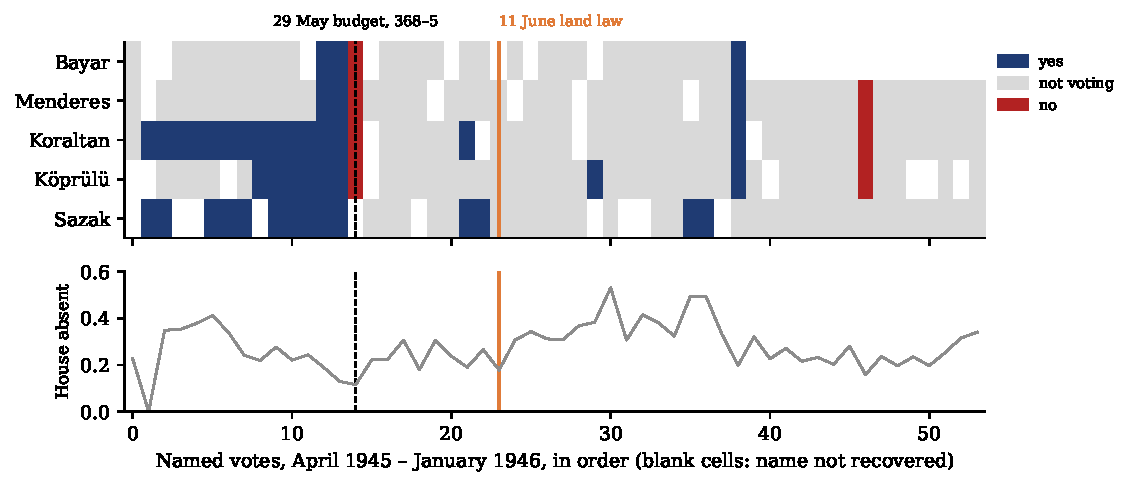
\includegraphics[width=\textwidth]{figA1_1945_withdrawal.pdf}
\caption{The Withdrawal of the Democrat Party Founders, 1945}
\label{fig:A1}
\begin{minipage}{\textwidth}\footnotesize
\textit{Note:} Top: each cell is one named vote, in order. Blank cells: the deputy's name was not recovered from the list. Bottom: share of non-excused deputies not voting. Dashed line: the seven-month budget of May 29, 1945 (368--5). Solid line: the land law of June 11, 1945 (345--0).
\end{minipage}
\end{figure}

\begin{table}[H]
\centering
\caption{The 1945 Land Debate: Principal Speakers and Verified Quotations}
\label{tab:A3}
\footnotesize
\begin{tabular}{L{4.2cm}L{2.1cm}cccrrr}
\toprule
\multicolumn{8}{l}{\textit{Panel A. Sixteen speakers with the most words (sessions 54--58 and 67--72)}} \\
Speaker & Province & Later DP & Farmer & Office & Turns & Words & Property share \\
\midrule
\tabinput{tables/ta3_debate.tex}
\bottomrule
\end{tabular}

\medskip
\begin{tabular}{L{3.1cm}L{2.6cm}L{10.2cm}}
\multicolumn{3}{l}{\textit{Panel B. Quotations (minutes file and page of the official PDF)}} \\
\toprule
Speaker & Date, source & Statement (translated) \\
\midrule
Adnan Menderes & 15.5.1945, 07017055 p.~22 & The bill's farmstead scheme is taken ``almost verbatim'' from the National Socialist hereditary farm law. \\
Refik Koraltan & 14.5.1945, 07017054 p.~30 & ``If the government continues on this path, I cannot trust it.'' \\
Cavit Oral & 4.6.1945, 07018067 p.~32 & ``The provisions of Article 17 recognize no limit in land.'' \\
Adnan Menderes & 4.6.1945, 07018067 p.~41 & Protests that the majority's motion on Article 17 was passed hand to hand for signatures and is adopted without debate; asks not to be counted against the land law. \\
Emin Sazak & 4.6.1945, 07018067 p.~46 & ``If I denied that my tie to land affects my speech and my feelings, I would be lying.'' \\
Emin Sazak & 5.6.1945, 07018068 p.~41 & ``Where are these serfs, these captives?'' \\
Refik Koraltan & 5.6.1945, 07018069 p.~7 & A unanimous vote on the law ``will be a clear answer'' to those who say there is opposition in the Assembly. (He did not vote.) \\
İbrahim Arvas & 13.3.1950, 08025063 p.~20 & At the CHP congress the delegates ``all at once attacked articles 15, 16, 17 and 43.'' \\
Şevket R. Hatipoğlu & 13.3.1950, 08025063 p.~25 & The 1945 law is ``the only legacy of honor I can leave my children.'' \\
Sabit Sağıroğlu & 13.3.1950, 08025063 p.~37 & Sharecropping arrangements ended ``all from the fear of Article 17.'' \\
Yahya Kanbolat (TİP) & 5.5.1966, mm02006092 p.~50 & Untitled land should be registered to its possessor only up to 100 dönüm of dry or 20 of irrigated land. \\
\bottomrule
\end{tabular}
\begin{minipage}{\textwidth}\footnotesize \textit{Note:} Panel A: speaker turns segmented from the minutes and matched to the 1943 roster. Office: speaking for the government or the committee. Property share: property and production terms as a share of property plus redistribution terms in the speaker's turns (a rough lexicon index; later-DP speakers 0.64, others 0.45, permutation $p=.17$). File prefixes: \texttt{tbmm} omitted. In March 1950 the agriculture minister presenting the dilution of the law was Cavit Oral (08025063 pp.~37--39).\end{minipage}

\end{table}

\subsection*{Part C. Tutelage, the Radical Flank, and Robustness}

Figure~\ref{fig:A2} shows the collapse of partisan distance on agrarian roll calls after the military memorandum of March 12, 1971. Figure~\ref{fig:A3} shows the salience of land reform in the minutes. Figure~\ref{fig:A4} reports the ideal-point maps for the remaining terms of the National Assembly. Table~\ref{tab:A4} sets out the comparison of land reform moments, the evidence on the radical flank, and robustness checks.

\begin{figure}[H]
\centering
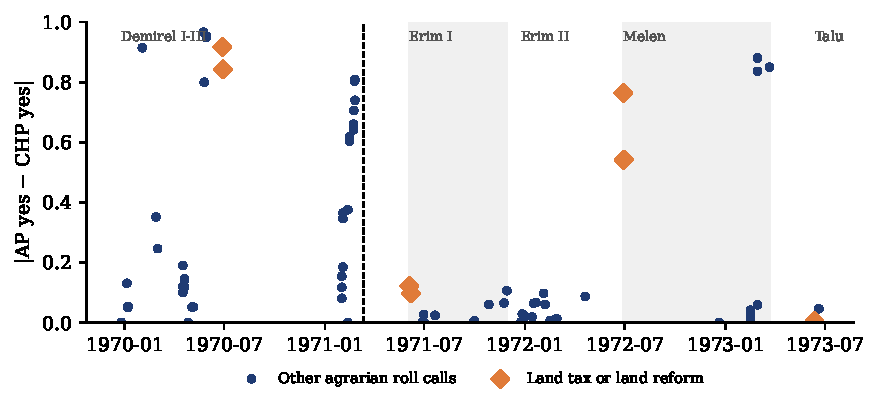
\includegraphics[width=.95\textwidth]{figA2_memorandum.pdf}
\caption{Partisan Distance on Agrarian Roll Calls, 1969--1973}
\label{fig:A2}
\begin{minipage}{\textwidth}\footnotesize
\textit{Note:} Each point is a National Assembly roll call: the absolute difference between the AP and CHP yes shares among votes cast. Bands mark cabinets; dashed line: the memorandum of March 12, 1971. The mean distance fell by 0.38 between the Demirel governments and the post-memorandum period; a placebo in time over 156 break dates in other terms gives $p=.03$.
\end{minipage}
\end{figure}

\begin{figure}[H]
\centering
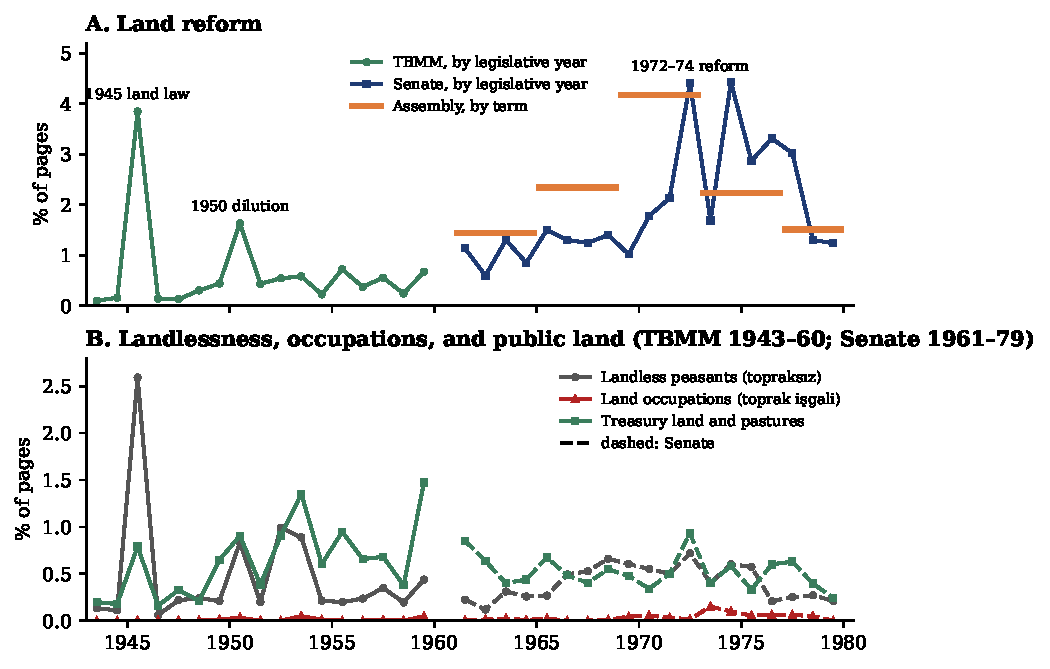
\includegraphics[width=.95\textwidth]{figA3_speech.pdf}
\caption{Land Reform in Parliamentary Speech, 1943--1980}
\label{fig:A3}
\begin{minipage}{\textwidth}\footnotesize
\textit{Note:} Share of pages of the minutes that mention land reform or land distribution (\textit{toprak reformu}, \textit{tarım reformu}, \textit{toprak dağıtımı}, \textit{topraklandırma}), by legislative year (single-chamber TBMM and Senate) and by term (National Assembly). Phrase counts from the text corpus.
\end{minipage}
\end{figure}

\begin{figure}[H]
\centering
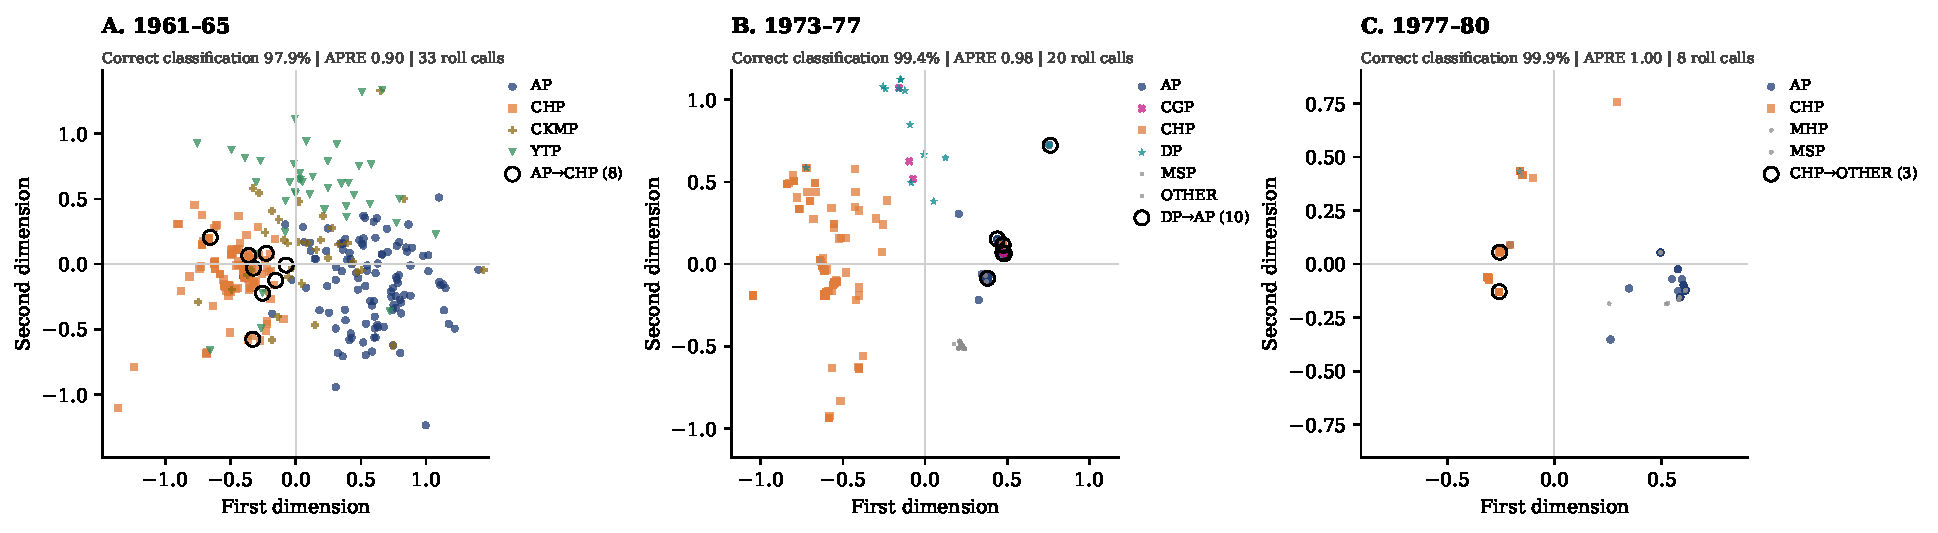
\includegraphics[width=\textwidth]{figA4_split_maps_other.pdf}
\caption{Estimated Positions of Deputies, National Assembly 1961--65, 1973--77, and 1977--80}
\label{fig:A4}
\begin{minipage}{\textwidth}\footnotesize
\textit{Note:} As Figure 1. Circled: deputies whose party at the end of the term differs from that at its start. Fewer agrarian roll calls meet the fitting criterion in 1973--80, so these positions rest on 20 and 8 roll calls.
\end{minipage}
\end{figure}

\begin{table}[H]
\centering
\begin{threeparttable}
\caption{Land Reform Moments, the Radical Flank, and Robustness}
\label{tab:A4}
\footnotesize
\begin{tabular}{L{3.0cm}L{4.1cm}L{3.1cm}L{4.8cm}}
\toprule
\multicolumn{4}{l}{\textit{Panel A. Moments when land reform reached a recorded vote}} \\
Moment & Regime & Recorded result & Opponents' action; outcome \\
\midrule
June 1945 & Single party (CHP) & Land law 345--0 & Voice in debate; founders' general withdrawal; \textbf{passed} \\
March 1950 & Two-party, election due & Dilution 261--15 & Critics rewrite law inside CHP (Oral minister); DP absent; \textbf{diluted} \\
1950--60 & DP majority & Titling and technical amendments only & No extension of distribution reached a vote; \textbf{shelved} \\
February 1965 & Coalitions & Motion 157--167 & AP mobilized (1.65$\times$ attendance), 98\% no; \textbf{defeated} \\
June 1973 & Military-supervised cabinets; TİP closed & Reform law 238--5 & AP 198--1 for; CHP 2 of 101 present; \textbf{passed} \\
\midrule
\multicolumn{4}{l}{\textit{Panel B. The radical flank: Workers' Party of Turkey (TİP), National Assembly 1965--69}} \\
\midrule
Roll calls & 78 & Outcome-pivotal & 0 (TİP's votes never decided an outcome) \\
Quorum-pivotal & 10 (9 passed) & Turnout of TİP & 37\% \\
Mean first dimension & TİP $-1.12$; CHP $-0.65$; AP $+0.34$ & Ceiling amendments (1966) & 100 dönüm dry / 20 irrigated; rejected by show of hands, no recorded vote \\
Quorum rule check & Outcome matches 226-of-450 rule in 289 of 295 roll calls & CHP $\rightarrow$ GP exit & $-0.04$ ($p=.46$) \\
\midrule
\multicolumn{4}{l}{\textit{Panel C. Robustness}} \\
\midrule
Farmer effect by era & 1946--50 $-0.005$ (0.010); 1950--60 $-0.001$ (0.008); 1961--65 $-0.012$ (0.013) & 1965--71 $+0.021$ (0.012); 1971--73 $0.000$ (0.020); 1973--80 $-0.001$ (0.008) & Within party and roll call; contested votes; SE clustered by deputy \\
Government premium, final passage, budgets, and accounts only & 1961--65 0.46; 1965--71 0.64 & 1971--73 0.35; 1973--80 0.84 & All stages: 0.42, 0.59, 0.31, 0.84 \\
1948 exit, alternative split date & January 1948: $+0.10$ & July 1948: $+0.10$ & Departure of the independent group vs.\ founding of the MP \\
1955 exit, all agrarian votes & $-0.16$ ($p<.001$) & Agency budgets: $-0.52$ & Stayers unchanged in both \\
1945 land law, later-DP absence & All 54 votes: DiD $+0.25$, $p=.07$ (votes), $p=.03$ (deputies) & After May 29 only: five founders $+0.21$ ($p=.18$); 14 later-DP $+0.15$ ($p=.15$) & Withdrawal general, not land-specific \\
DID$_M$ placebo & 0.002 [0.000, 0.010] & Turnout placebo 0.03 & Periods without status switches \\
\bottomrule
\end{tabular}
\begin{tablenotes}\footnotesize
\item \textit{Note:} Panel A: see text and Figure 4. Panel B: outcome-pivotal means that reversing TİP's votes would change the result; quorum-pivotal means that TİP's presence or absence decided whether 226 deputies took part. Panel C: estimates as in the main tables with the stated changes.
\end{tablenotes}
\end{threeparttable}
\end{table}


\end{document}
